\documentclass[10pt]{article}

%-------Packages---------
\usepackage{enumerate}
\usepackage[margin=0.75in]{geometry}
\usepackage{rotating}
\usepackage{hyperref}
\usepackage{verbatim}

\bibliographystyle{plain}

%--------Meta Data: Fill in your info------
\title{Website Changes and User Behavior: \\
Using Panjiva Data to Examine Code Changes}
\date{\today}
\author{John Wang \\
14.27 Final Paper}


\begin{document}

\maketitle

\abstract{Most software developers implicitly believe that change tends to improve a website. However, the story seems far more complicated. This paper examines how code changes affect user behavior on the internet by analyzing a particular website, \url{http://www.panjiva.com} and its database of activity logs. The paper identifies some factors which affect how code changes influence user activity levels and finds patterns in how users respond to change. Users tend to increase their repeat usage when code changes are of high quality and when the changes affect portions of a website which users already frequent. Users respond negatively to changes in areas of the website with low traffic. A massive volume of code change, in general, does not necessarily lead to higher user activity on a website and in fact may negatively impact the user experience.}  

\tableofcontents

\newpage

\section{Introduction}

Silicon Valley has historically been built on constant change. Indeed, one of the tenets of technology companies and web-based startups is the idea of change. For example, Facebook's official motto is ``Move fast and break things.''  However, few people have examined the effects of website and product changes on user activity. Do users tend to respond favorably to website changes? Moreover, how do users react to different types of changes? Can different characteristics of users change how users respond to certain changes?

All of these questions are crucial and allow developers to create better websites and tools for their users. This paper examines the effects of code changes on user activity. In particular, the paper focuses on the short term effects of everyday changes to a website. The paper exploits a unique dataset and examines how short-term user activity (both overall on the entire website and on a more granular, per-user level) are affected by code changes. The unique dataset comes from Panjiva, Inc., which provided the author access to its entire database.

\section{Dataset Explanation}

The proprietary dataset used in this paper comes from the back-end databases collected by Panjiva, Inc. Panjiva's website \url{http://www.panjiva.com} acts as a medium for buyers and suppliers of manufactured goods. The site provides a communication platform so that bulk buyers of a particular good can search and obtain unbiased information on factories and suppliers of that good. These two parties can then communicate and send messages over Panjiva's interface, attempting to strike a deal. 

Panjiva's competitive advantage rests in its ability to parse government import and export data in order to obtain unbiased information about suppliers. Panjiva determines a supplier reliability score and also provides recent history of a supplier's shipments, and allows buyers to search and aggregate this information easily. Most firms that use Panjiva are large to medium size buyers of components. For example, a department store would use Panjiva to search for suppliers of shirts or clothing, or a home improvement store would search for suppliers of socket wrenches. In addition, Panjiva provides data on trends in global manufacturing and shipping by leveraging the government data it already mines for individual supplier information.

The dataset used in this paper comes from the event and activity logs of Panjiva's website. Each time a user performs some significant event or activity on the Panjiva website, an entry will be created in either the event or activity log. If the user has a registered account with Panjiva, the action will be recorded in the activity logs. All activities, regardless of whether a user has an account, are recorded in the event logs. All nontrivial features of the website, including supplier search, U.S. import and export search, and profiles views, are accounted for and stored in a SQL database.

The data in the event and activity logs are organized so that one can trace the exact user or subscribed account for which the entry. In particular, the logs contain information on the ip address of the user, the time the activity was performed, the webpage the activity occurred on, and extra data depending on the type of activity performed. 

The enormous quantity and granularity of this data enable the analysis of user-level interactions. The event logs contain about 124 million entries while the activity logs contain about 13 million entries. Moreover, the data in each of these logs extends for multiple years, allowing one to analyze the growth of Panjiva as a company and the effect of different changes to the website.

\subsection{Summary Statistics}

Summary statistics providing an overview of Panjiva's business and website are provided in table \ref{table:panjiva-overview}. Panjiva was incorporated in 2008 and has since developed a customer base composed mostly of buyers of manufactured goods. The website provides free services (a limited number of searches) for free users, and provides many more services to subscribers (there are multiple levels of subscription). 

\begin{table}[h!]
\centering
\caption{Panjiva Overview}
\begin{tabular}{l || l}
\hline
Total Users & 121,653 \\
Subscribing Users & 2,985 \\
Monthly Site Visits & 903,426 \\
Monthly Unique Visitors & 762,723 \\
Average Pages per Visit & 1.99 \\
Average Visit Duration & 1 min 18 sec \\
\hline
\end{tabular}
\label{table:panjiva-overview}
\end{table}

Commits can be thought of as changes to the code. In each commit, a software developer will introduce new code or delete old code which will then be launched to the production website. Typically a single developer at Panjiva will commit a couple of times throughout the workday. Figure \ref{fig:commit-history} shows a histogram of the number of commits throughout a 52 week period ending on 11/24/2012. Commit activity varies depending on the season and the week. In particular, commits during the summer spike upwards and there will be one or two weeks each quarter when commits fall to low levels. The second phenomenon is due to the fact that Panjiva holds a quarterly retreat where engineers reflect upon the work done over the quarter. Typically the amount of code written decreases during these weeks. 

\begin{figure}[h!]
\centering
\caption{52-Week Commit Activity}
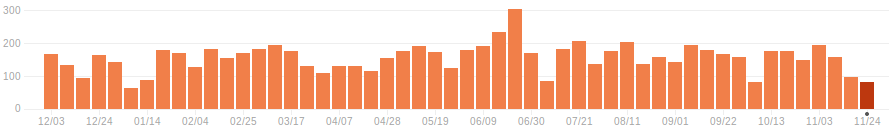
\includegraphics[width=5in]{pictures/commit-activity.png}
\label{fig:commit-history}
\end{figure}

Table \ref{table:commit-stats} shows statistics on a snapshot of the commit repository made on 11/25/2012. The table shows an enormous number of changes throughout the history of the website. In addition, the 1.3 million lines of code show that one can use the variation in the lines of code that a commit changes in order to better understand how each commit affects user behavior.

\begin{table}[h!]
\centering
\caption{Overall Commit Statistics - 11/25/2012}
\begin{tabular}{l || l }
\hline
Active Days (at least 1 commit) & 1,983 \\
Total Current Files & 20,901 \\
Total Lines of Code & 1,313,235 \\
Total Lines of Code Added & 3,989,295 \\
Total Lines of Code Removed & 2,676,060 \\
Total Commits & 29,924 \\
Total Authors/Developers & 33 \\
\hline
\end{tabular}
\label{table:commit-stats}
\end{table}

Examining commits in more detail, one can see that the majority of commits occur during working hours (from 11am to 6pm EST). Moreover, each day is fairly regular in the number of commits that occur. Commits are at a high level throughout the work day, and fall off to a low, relatively constant level throughout the night. Figure \ref{fig:commit-hours} shows the times of day during which commits happen the most frequently. 

\begin{figure}[h!]
\centering
\caption{Commit Frequency by Time of Day}
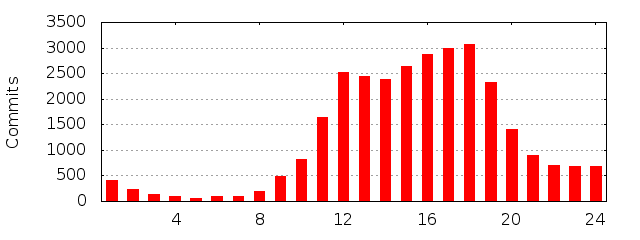
\includegraphics[width=4in]{pictures/commit-hours.png}
\label{fig:commit-hours}
\end{figure}

Finally, note that almost no commits occur on weekends. Only 5\% of the commits happen on either Saturday or Sunday.

\section{Macro-Level Results}

This section examines how code changes affect the total amount of user activity across the entire website (macro-level effects). In particular, this section analyzes the change in a number of metrics of user activity controlling for the amount of code changed in a particular day. The regression specification used will the as follows:

\begin{eqnarray}
y^i_{t} = c_0 + \bar{\gamma}^T \bar{M}_t + \bar{\beta}^T \bar{\chi}_t + \epsilon_t
\end{eqnarray}

Where $t$ indexes day, $y^i_t$ corresponds to the $i$th metric of user activity on day $t$, $\bar{M}_t$ corresponds to a vector of covariates that represent changes in the code, $\bar{\chi}_t$ is a vector of controls, and $\epsilon_t$ is an error term. We will use a number of different metrics for user activity and the specification will be run with each of them. 

The first two metrics for user actions are the total number of entries in the activity or event logs for a particular time period. Recall that event logs are database records for actions performed by anyone, while activity logs are records for only those users who have a registered account with Panjiva.

Another set of metrics are the total number of distinct users performing either activities or events in a given time period. Finally, one might also use the average number of actions per user, whether action is defined using records from activity or event logs. One would expect the each of these metrics to measure a different aspect of user behavior. 

\subsection{Daily Effects of Code Changes}

Table \ref{table:macro-action-results} displays the results from using the total action count as a metric for user activity. The regressions in table \ref{table:macro-action-results} attempt to find the effect of different changes in the code base on different measures of user activity. A commit can be measured by the number of files it changes, or the number of lines of code it changes. Changes in lines of code can be either insertions or deletions. Each of these measures is percentilized (sorted rank is divided by the total number of observations). The regressions below are performed on aggregated statistics per day, with a dummy variable equal to 1 on the weekends and 0 otherwise.  

\begin{sidewaystable}[p]
\centering
\caption{Effect of Commits on User Activity}
{
    \def\sym#1{\ifmmode^{#1}\else\(^{#1}\)\fi}
    \begin{tabular}{l*{6}{c}}
    \hline\hline
        &\multicolumn{1}{c}{(1)}&\multicolumn{1}{c}{(2)}&\multicolumn{1}{c}{(3)}&\multicolumn{1}{c}{(4)}&\multicolumn{1}{c}{(5)}&\multicolumn{1}{c}{(6)}\\
        &\multicolumn{1}{c}{activitylogcount}&\multicolumn{1}{c}{eventlogcount}&\multicolumn{1}{c}{activitylog}&\multicolumn{1}{c}{eventlog}&\multicolumn{1}{c}{avguseractivity}&\multicolumn{1}{c}{avguserevents}\\
        &\multicolumn{1}{c}{}&\multicolumn{1}{c}{}&\multicolumn{1}{c}{distinctusercount}&\multicolumn{1}{c}{distinctusercount}&\multicolumn{1}{c}{}&\multicolumn{1}{c}{}\\
        \hline
        fileschangedpercentile&     -5530.7         &    -60589.4\sym{*}  &       460.5         &       492.7         &      -10.40\sym{*}  &      -148.6         \\
        &     (-1.91)         &     (-2.26)         &      (0.65)         &      (0.71)         &     (-2.01)         &     (-1.52)         \\
        [1em]
        insertionspercentile&      4868.8\sym{*}  &     47053.7\sym{*}  &       284.2         &       118.6         &       2.817         &       79.92         \\
        &      (2.12)         &      (2.22)         &      (0.51)         &      (0.22)         &      (0.69)         &      (1.03)         \\
        [1em]
        deletionspercentile&      2778.9         &     29970.6         &      -192.2         &      -184.4         &       4.670         &       49.47         \\
        &      (1.29)         &      (1.50)         &     (-0.36)         &     (-0.36)         &      (1.21)         &      (0.68)         \\
        [1em]
        weekend     &    -14708.0\sym{***}&    -79769.8\sym{***}&     -1060.6\sym{***}&      -816.2\sym{***}&      -0.297         &       257.0\sym{***}\\
        &    (-16.48)         &     (-9.65)         &     (-4.86)         &     (-3.82)         &     (-0.19)         &      (8.49)         \\
        [1em]
        \_cons      &     22396.6\sym{***}&    224482.8\sym{***}&      1635.7\sym{***}&      1395.9\sym{***}&       25.00\sym{***}&       340.6\sym{***}\\
        &     (25.05)         &     (27.12)         &      (7.49)         &      (6.52)         &     (15.58)         &     (11.24)         \\
        \hline
        \(N\)       &         474         &         475         &         474         &         475         &         474         &         475         \\
        \hline\hline
        \multicolumn{7}{l}{\footnotesize \textit{t} statistics in parentheses}\\
        \multicolumn{7}{l}{\footnotesize \sym{*} \(p<0.05\), \sym{**} \(p<0.01\), \sym{***} \(p<0.001\)}\\
        \multicolumn{7}{l}{The table provides regression estimates of how different measures of user actions vary with changes in the codebase.}\\
        \multicolumn{7}{l}{The table was created by aggregated data from the Panjiva activity and event logs over the period from 7/14/2011}\\
        \multicolumn{7}{l}{to 11/24/2012. Variables are broken apart by day, so that counts are per day. Activity logs record information}\\
        \multicolumn{7}{l}{about users with registered accounts, while event logs record information about all users regardless of whether they}\\
        \multicolumn{7}{l}{have registered with the Panjiva.}\\
        \\
        \multicolumn{7}{l}{Activitylogcount and eventlogcount aggregate the total number of records seen per day in the activity and event logs}\\
        \multicolumn{7}{l}{respectively. Activitylogdistincusercount and eventlogdistinctusercount aggregate the number of distinct users that}\\
        \multicolumn{7}{l}{have performed an action in either the activity or event logs respectively. Finally, avguseractivity and avguserevents}\\
        \multicolumn{7}{l}{divides the total number of records by the total number of distinct users per day to arrive at an average number of}\\
        \multicolumn{7}{l}{actions per day.}\\
        \\
        \multicolumn{7}{l}{Weekend is a dummy variable equal to 1 if the day is a Saturday or Sunday and 0 otherwise. The other covariates are}\\
        \multicolumn{7}{l}{percentilized by sorting each day and taking the rank and dividing by the total number of days. Files changed, insertions}\\
        \multicolumn{7}{l}{and deletions are obtained from commit history and are aggregated over each day. Insertions and deletions are the}\\
        \multicolumn{7}{l}{total number of lines of code inserted or deleted, respectively.}
        \end{tabular}
}
\label{table:macro-action-results}
\end{sidewaystable}

The table shows the effect of commits on same day user activity. In general, changes to the code have minor and insignificant effects on metrics derived from the event logs. There are only significant effects for the eventlogcount. However, code changes have a stronger effect on metrics derived from the activity logs. Notice that for activitylogcount, the insertionspercentile variable is significant and the fileschangedpercentile and deletionspercentile are within the 10\% significance level. Moreover, fileschangedpercentile has a significant effect on the average number of activities per user. The number of files changed and number of insertions are the only significant regressors, and they have opposing signs. 

Increasing the number of files changed tends to decrease user activity, while increasing the number of code insertions tends to increase user activity. Although this result seems perplexing, there are a number of possible explanations. First, it is possible that the commits which change fewer files tend to be higher quality commits. Thus, if a commit touches a large number of files, there is a higher likelihood that this commit would introduce a bug or contain low quality changes. However, it seems that introducing new code, instead of deleting code, has a positive effect on user activity, controlling for the number of files changed. 

Another, though possibly less satisfying explanation, is that code changes hurt average user activity in general. Since average user activity provides a measure of the organic growth of the website, it may be a better measure for the effects of code changes. Note that increasing total user count could result from a large number of new distinct user performing one or two actions each on the website. Although this could be construed as an increase in activity, each user could leave quickly, which would negatively affect long term traffic. Thus, one can think of the negative coefficient on the fileschangedpercentile variable as decreasing the long-term user activity with more code changes.

However, the second explanation seems unlikely because of the fact that code changes are constantly occuring. The regression is measuring the marginal effect of commits. Each additional file changed could provide a negative effect due to diminishing returns. Thus, one could have a negative coefficient on fileschangedpercentile even when increasing the number of files changed at very low levels (i.e. from 0 to 1) would increase user activity.

Also, notice that commits have no significant effect on the total number of distinct users. This is unsurprising since it is likely that it takes a significant period of time to increase the number of distinct users. Changes to the website will probably not spill over to other users during short time spans (like a day). Users do not have the time yet to share their new experiences on the site, so each user can be thought of as independent of others during these short time periods. Therefore, it is unsurprising that code changes fail to increase the total number of distinct users on the website. 

\subsection{Lagged Effects of Code Changes}

Note that the analysis of the previous section uses the implicit assumption that for a given day $t$, only the code changes on day $t$ influence user actions on day $t$. The previous regression assumes first that there is no lag between a code change and the change in user activity resulting from the code change, and second that only a single day's code changes affects the user activity on day $t$. Both of these assumptions are simplifications, and this section will relax the first one.

The original specification of the regression will now depend upon $y^i_{tx}$, where $x$ is a number of days of lag. Thus, if $x = 5$, then $y^i_{tx}$ will correspond to the $y^i_{t}$ which was five days ahead in the original specification. The specification will be run for all $x$ in some range $[0, R]$ to identify whether code changes have a lagged effect upon the changes in user activity. Figure \ref{fig:avg-events-time-coefficients} shows the change in the coefficients of fileschangedpercentile (in red) and lineschangedpercentile (in blue) with lags of $x \in [1, 30]$ when the regressor is average events per user from the event logs. Figure \ref{fig:avg-activities-time-coefficients} provides the same information for the regressor of average activities per user from the activity logs. 

The coefficient plotted in these figures is the $\gamma$ coefficient from the following specification (where $x$ varies from 1 to 30):
\begin{eqnarray}
y^i_{tx} = c_0 + \gamma M_{t} + \beta weekend_{t} + \epsilon_t
\end{eqnarray}

Like the previous specification, $M_t$ is a measure of code change in day $t$ (either fileschangedpercentile or lineschangedpercentile) and $weekend_t$ is a dummy variable equal to 1 if $t$ represents a day which is either Saturday or Sunday. Each figure plots the $\gamma$ coefficient (on the y-axis) from the above regression with different time lags ranging from 0 to 30 (on the x-axis).

\begin{figure}[h!]
\caption{$\gamma$ Coefficients with Varying Lags, Regressed on Average Event Logs per User}
\centering
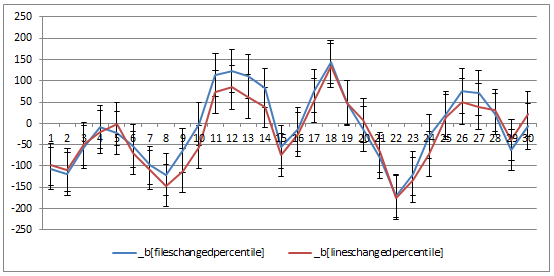
\includegraphics[width=5in]{pictures/avg_events_time_coefficients.png}
\label{fig:avg-events-time-coefficients}
\end{figure}

Examining figure \ref{fig:avg-events-time-coefficients}, it is difficult to ascertain the actual effect of the change in time lags (note that error bars correspond to standard errors). Both covariates representing code changes, fileschangedpercentile and lineschangedpercentile, have very similar coefficients across different time lags. Small time lags less than 10 result in negative and significant coefficients for both fileschangedpercentile and lineschangedpercentile, while larger time lags tend to have positive and significant coefficients. The second trend, however, is bucked by a couple of negative coefficients when $x \in [21, 24]$. 

The amount of noise inherent in the event logs probably makes the graph difficult, if not impossible, to interpret. One could hypothesize that the shape of the curve in figure \ref{fig:avg-events-time-coefficients} suggests that code changes have differential effects depending on the amount of time lag one accounts for. However, this explanation seems week since event logs contain records of all possible users, making it difficult to interpret overall changes in the trend without decomposing into well-defined groups of users. Second, figure \ref{fig:avg-activities-time-coefficients} shows that the same results performed on the action log records provides substantially more elucidating results.

\begin{figure}[h!]
\caption{$\gamma$ Coefficients with Varying Lags, Regressed on Average Activity Logs per User}
\centering
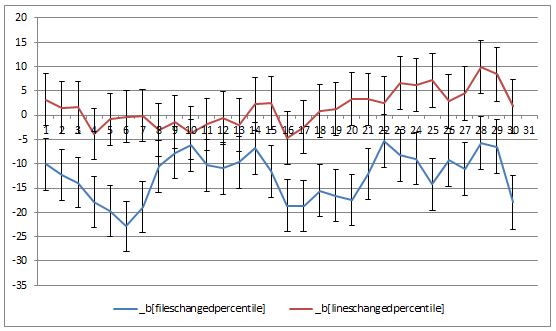
\includegraphics[width=5in]{pictures/avg_activities_time_coefficients.png}
\label{fig:avg-activities-time-coefficients}
\end{figure}

Figure \ref{fig:avg-activities-time-coefficients} shows large and consistent negative coefficients on fileschangedpercentile with all different ranges of lag. The figure also shows that the coefficient on lineschangedpercentile is not significantly different from zero for almost all lags, suggesting that it has little effect in predicting user activity. 

However, the number of files changed per day has a significant and negative coefficient throughout all time lags, reinforcing the results from the previous section that the more files changed on a particular day, the lower user activity tends to be. This result stays consistent across time, suggesting that lower user activity begins early and persists for a number of days. This provides more evidence that increasing the number of files changed per day, given the current number of files changed, will decrease user average user activity from users who are registered on Panjiva. 

\begin{figure}[h!]
\caption{$\gamma_0$ and $\gamma_1$ Coefficients with Varying Lags. Regressed on Average Activity Logs per User, the graph displays the coefficients on insertionspercentile and deletionspercentile as time lags range from 0 to 30.}
\centering
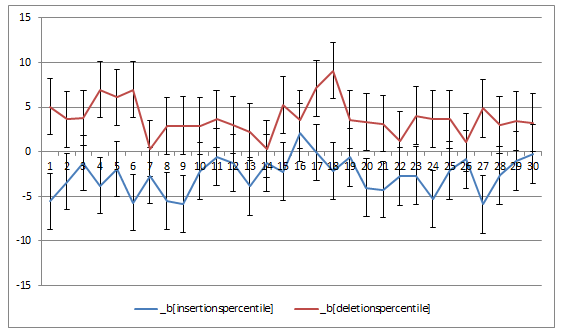
\includegraphics[width=4.5in]{pictures/commit_percentiles_time_coefficients.png}
\label{fig:insertions-deletions-time-coefficients}
\end{figure}

Figure \ref{fig:insertions-deletions-time-coefficients} examines the change in average user activity due to insertions and deletions of code. This graph makes the behavior of coefficients on insertionspercentile and deletionspercentile from the original regressions more clear. The figure displays the $\gamma_0$ and $\gamma_1$ coefficients from the following regression:
\begin{eqnarray}
avguseractivity_{tx} = c_0 + \gamma_0 insertionspercentile_t + \gamma_1 deletionspercentile_t + \beta weekend_t + \epsilon_t
\end{eqnarray}

The graph remains consistent across different levels of lags-insertionspercentile's coefficient tends to be negative while deletionspercentile's coefficient tends to be positive. Although there exist multiple lags for which either $\gamma_0$ or $\gamma_1$ is not significantly different from 0, it is never the case that the $\gamma_0$ and $\gamma_1$ coefficients switch sign. This implies that the actual effect of increasing the insertion percentile is likely correlated with lower average user activity while increasing the deletion percentile does the opposite.

This finding seems to imply that removing code tends to be better than adding code. Although this hypothesis was reached on macro-level data, it is still an interesting idea. Perhaps removing code is correlated with making better code, and inserting new code usually happens with a new, possibly buggy feature being added. If this is the case, then it seems that users respond better to clean, non-buggy code. To investigate this further, regressions are performed on a more granular level.

\section{Micro-Level Results}

Although the macro-level regressions provided some insight into how code changes affect user activity, they really could not provide anything more than correlations. Complex factors could have been governing the relationship between code changes and user activity, and only weekend dummies were included in the regressions. Thus, the macro-level results must be taken with a grain of salt since the correlations observed could be brought through completely different mechanisms than the ones suggested. 

However, the micro-level dataset can be much more powerful in its results. The dataset used in this section exclusively uses the activity logs, and exploits the fact that each recorded activity comes with a unique user identification tag and timestamp. Therefore, it is possible to know exactly when a user was visiting a given page. 

Even better, most of the code changes made throughout the day can be thought of as exogeneous shocks. This arises from the fact that almost none of the releases made by developers are announced to the user base beforehand. Even if the changes are announced, few users would be notified and aware of the change because Panjiva typically advertises such changes through its blog. Less than 1\% of Panjiva's total pageviews come from its blog, so it is safe to assume that most users are unaware of any planned changes to the website. Since these code changes can be thought of as exogeneous with a high degree of accuracy, one can develop an empirical approach that examines the shock induced by each code change.

\subsection{Search Controller}

The search page has always been Panjiva's most trafficked page. Possibly due to this, it has received a number of code changes, both in terms of back-end structure and also in terms of the user interface. There is, correspondingly a large amount of variation in the number of lines of code changed and the times at which code was changed on the search page. To exploit this variation, this section will examine user activity before and after a code change. 

In particular, this section limits the activity log dataset to only users who have seen the search page both two days before and after a particular change. Thus, for each code change in the search page, the users that had recently seen the unchanged page and also the changed page were examined. Any users seeing the search page over two days before the change were dropped, as were users who saw the search page over two days after the change. User activity was measured with the $num_views_day_after$ variable, which corresponds to the number of views of the search page in the day after the current view of the page. Note that day after is defined as 86,400 seconds after the original view occurred. 

Since the dataset was confined to only users who saw both the original website and the changed website, one can take the difference between the number of views before and after the change as the effect of the change (assuming that commits are exogeneous). Another refinement made to the dataset is that only commits to the search controller were examined.\footnote{A controller in a Model-View-Controller web framework is typically the piece of the code that manages the data and sends it along to the user interface. For Panjiva, almost all of the heavy-lifting is done in the controller (this includes data processing and the search algorithm itself).} This choice was made because a significant portion of the user interface code is antiquated and left in the code-base. Therefore, large changes to the user interface code could spuriously affect parts of the code that no longer are seen on the production website. 

The time period from 7/14/2011 until 11/25/2012 was examined (to confine the dataset to more recent changes). A total of 294 changes occurred during this time, ranging from small one line changes to larger changes in hundreds or thousands of lines. The following regression specification was used:
\begin{eqnarray}
num\_views\_day\_after_{it} = c_0 + \beta_0 \mu_{it} + \beta_1 hour\_dummies_{it} + \epsilon_{it}
\end{eqnarray}

Where $i$ indexes the $i$th commit and $t$ indexes the $t$th view in the 4 day window surrounding the $i$th commit. Here $\mu_{it}$ is either a dummy variable $after\_commit$ which is equal to 1 if the view of the search page occurred after the commit and 0 otherwsie, or it is equal to $time\_from\_event$ which is the number of seconds since the commit. Therefore, if a view of the search controller occured at time $T_1$ and the commit occurred at time $T_2$, then $time\_from\_event = T_1 - T_2$.  

\begin{table}[h!]
\caption{Search Controller Micro-Level Results}
\centering
{
    \def\sym#1{\ifmmode^{#1}\else\(^{#1}\)\fi}
    \begin{tabular}{l*{4}{c}}
    \hline\hline
        & \multicolumn{4}{l}{Dependent Variable: num\_views\_day\_later} \\ 
        &\multicolumn{1}{c}{(1)}&\multicolumn{1}{c}{(2)}&\multicolumn{1}{c}{(3)}&\multicolumn{1}{c}{(4)}\\
        \hline
        after\_commit&       5.541\sym{***}&               &       3.378\sym{***}&                     \\
        &     (17.91)         &                     &     (11.20)         &                     \\
        [1em]
        time\_from\_event&                     &   0.0000737\sym{***}&                     &    0.000110\sym{***}\\
        &                    &     (43.76)         &                     &     (66.60)         \\
        [1em]
        created\_at\_hour&             No        &           No           &       Yes &      Yes \\
        dummies?&                     &                     &              &            \\
        [1em]
        \_cons      &       156.9\sym{***}&       159.9\sym{***}&       138.3\sym{***}&       139.7\sym{***}\\
        &    (731.32)     &   (1033.47)         &    (127.71)         &    (130.50)         \\
        \hline
        \(N\)       &     2345617       &     2345617         &     2345617         &     2345617         \\
        \hline\hline
        \multicolumn{5}{l}{\footnotesize \textit{t} statistics in parentheses}\\
        \multicolumn{5}{l}{\footnotesize \sym{*} \(p<0.05\), \sym{**} \(p<0.01\), \sym{***} \(p<0.001\)}\\
        \multicolumn{5}{l}{Regression using micro-level dataset. Confined only to users who saw the} \\
        \multicolumn{5}{l}{search page both before commit $i$ and after commit $i$ inside of a 4 day}\\
        \multicolumn{5}{l}{window surrounding the time of the commit. The num\_views\_day\_later} \\
        \multicolumn{5}{l}{variable contains the number of views of the search page for each user one}\\
        \multicolumn{5}{l}{day after the record was created. Commits are confined only to changes in} \\
        \multicolumn{5}{l}{the search controller.} 
        \end{tabular}
}
\label{table:search-micro-commit-results}
\end{table}

There are about 2.3 million observations in this refined dataset and table \ref{table:search-micro-commit-results} shows the regression results of the specification defined above. The table shows that actions recorded after the commit occurs have a significantly higher number of views. Moreover, the positive coefficient on the time\_from\_event variable shows that as one gets further away from the commit time, the number of views of the search page increases. Thus, the number of views that occur after the commit is greater than the number of views before the commit (since time\_from\_event is negative before a commit and positive afterwards). The coefficients on after\_commit and time\_from\_event are strongly statistically significant (much higher than normal levels), which suggests that commits have a large positive effect on user actiivty. 

The statistical significance remains even when hour dummies are included (a set of 24 dummy variables where created\_at\_hour\_i = 1 if the activity record was created in the $i$th hour of the day and 0 otherwise). This provides strong evidence that code changes in the search controller significantly affect user behavior. Since commits are most likely exogeneous, user activity seems to increase significantly due to the changes in the search controller. 

\subsection{Insertions and Deletions}

However, it is still unclear from these regressions why user activity increases. To examine this in more detail, a regression with the following specification was conducted:
\begin{eqnarray}
num\_views\_day\_later_{it} &=& \beta_0 after\_commit_{it} + \beta_1 insertionspercentile_{it} + \beta_2 deletionspercentile_{it} \\ \nonumber
&+& \beta_3 insertionspercentile_{it} * after\_commit_{it} \\ \nonumber
&+& \beta_4 deletionspercentile_{it} * after\_commit_{it} \\ \nonumber
&+& \beta_5 hour\_dummies_{it} + c_0 +  \epsilon_{it}
\end{eqnarray}

Here, the specification uses interaction terms between the after\_commit dummy variable and the insertion and deletion percentile variables. Using the interaction coefficients, one can determine the additive effect of insertion an extra line of code on the change in the number of views after the commit. Looking on the $\beta_3$ and $\beta_4$ coefficients in the above specification will tell one how much additive effect on the number of views there is when a commit increases the insertion or deletion percentile (respectively) by 1 after a commit. In essence, it measures the effect of inserting or deleting lines of code on how users will respond to a change.  

Table \ref{table:commit-percentiles-micro} displays the results of the above specification with and without the hour dummies, and also with different sets of controllers. The regressions in columns 1 and 2 of table \ref{table:commit-percentiles-micro} use observations confined to users who saw changes in the search controller. Columns 3 and 4 use the same specification, but include observations from seven other controllers as well. These controllers are the communication, customs, my\_panjiva, profile, project, us\_exports, and us\_imports controllers. Each of these controllers corresponds to a different landing page on the Panjiva website.

Including all of the controllers almost doubles the number of observations available at 3.8 million. However, the results with different controllers mirror the results found just in the search controller. In particular, the interaction term coefficients ($\beta_3$ and $\beta_4$ from the specification) tend to be similar across all the regressions. More insertions in the codebase increase the positive effect of a code change on user activity. One sees that $\beta_3$, which corresponds to the coefficient on the interaction between an increase in the insertions percentile and the after\_commit variable, is large, positive, and highly statistically significant. 

This implies that insertions in the code tend to increase the number of views a user will have on a particular page $p$ of the site, with respect to how much that user viewed $p$ before the code change. Deletions in the code tend to have the opposite effect, though this seems to depend on the controller affect. Although the negativitiy of $\beta_4$ is highly statistically significant on only the search controller, it loses its significance once all controllers are included in the regression in columns 3 and 4. However, one can say that deletions in the code, at least in the search controller, have a significant negative effect on the number of pages a user will view in the future.

\begin{sidewaystable}[p]
\centering
\caption{Types of Commits and User Responses to Code Changes}
{
    \def\sym#1{\ifmmode^{#1}\else\(^{#1}\)\fi}
    \begin{tabular}{l*{4}{c}}
    \hline\hline
        &\multicolumn{1}{c}{(1)}&\multicolumn{1}{c}{(2)}&\multicolumn{1}{c}{(3)}&\multicolumn{1}{c}{(4)}\\
        &\multicolumn{1}{c}{num\_views\_day\_later}&\multicolumn{1}{c}{num\_views\_day\_later}&\multicolumn{1}{c}{num\_views\_day\_later}&\multicolumn{1}{c}{num\_views\_day\_later}\\
        \hline
        after\_commit&      -10.86\sym{***}&      -13.79\sym{***}&      -325.5\sym{***}&      -305.9\sym{***}\\
        &    (-16.90)         &    (-22.03)         &   (-154.63)         &   (-149.28)         \\
        [1em]
        insertionspercentile&      -50.97\sym{***}&      -50.76\sym{***}&      -650.6\sym{***}&      -609.5\sym{***}\\
        &    (-54.12)         &    (-55.34)         &   (-218.09)         &   (-209.88)         \\
        [1em]
        deletionspercentile&       66.31\sym{***}&       63.35\sym{***}&       251.5\sym{***}&       230.8\sym{***}\\
        &     (70.67)         &     (69.34)         &     (84.73)         &     (79.94)         \\
        [1em]
        insertionspercentile *&       57.00\sym{***}&       58.05\sym{***}&       393.0\sym{***}&       365.1\sym{***}\\
        after\_commit&     (41.21)         &     (43.09)         &     (89.07)         &     (85.01)         \\
        [1em]
        deletionspercentile * &      -24.16\sym{***}&      -23.64\sym{***}&       2.306         &       3.295         \\
        after\_commit&    (-17.65)         &    (-17.74)         &      (0.53)         &      (0.77)         \\
        [1em]
        created\_at\_hour&      No               &    Yes &          No           &     Yes\\
        dummies?&                     &            &                     &      \\
        [1em]
        Controllers Used&      Search               &    Search &         All           &     All\\
        &                     &            &                     &      \\
        [1em]
        \_cons      &       150.1\sym{***}&       133.2\sym{***}&       606.5\sym{***}&       491.0\sym{***}\\
        &    (336.67)         &    (116.37)         &    (420.98)         &    (130.17)         \\
        \hline
        \(N\)       &     2345617         &     2345617         &     3858943         &     3858943         \\
        \hline\hline
        \multicolumn{5}{l}{\footnotesize \textit{t} statistics in parentheses}\\
        \multicolumn{5}{l}{\footnotesize \sym{*} \(p<0.05\), \sym{**} \(p<0.01\), \sym{***} \(p<0.001\)}\\
        \multicolumn{5}{l}{Set of regressions which examine the effect of insertions and deletions in the code on the number of views that a}\\
        \multicolumn{5}{l}{user will have on page $p$ in the one day time span after viewing page $p$. The after\_commit variable is equal to}\\
        \multicolumn{5}{l}{if the current observation occurs after the commit that it corresponds to. All observations are within a four day}\\
        \multicolumn{5}{l}{window of the commit (2 days before and 2 days after) and contain only users who have seen page $p$ both before the}\\
        \multicolumn{5}{l}{commit and after the commit.}\\
        \multicolumn{5}{l}{The variables insertionspercentile and deletionspercentile are calculated as the percentile rank of the number of}\\
        \multicolumn{5}{l}{insertions and deletions for the current commit, respectively. The created\_at\_hour dummies correspond to dummies}\\
        \multicolumn{5}{l}{equaling 1 if the hour is equal to $i$ and 0 otherwise for $i \in [1,24]$.}\\ 
        \multicolumn{5}{l}{The dataset is either confined to the search controller, or uses all the controllers in the following list:}\\
        \multicolumn{5}{l}{communication, customs, my\_panjiva, profile, project, us\_exports, and us\_imports controller.}
        \end{tabular}
}
\label{table:commit-percentiles-micro}
\end{sidewaystable}

\subsection{Differential Controller Effects}

One might also want to examine how users change their behaviors depending on the controller for which a change is made. Perhaps users react differently to changes in different controllers. For example, the search controller is the most heavily used and is the controller that is most frequently a ``return controller'' (a page that a user will repeatedly visit). However, other controllers tend to be visited less often and tend not to be repeatedly visited. One would expect that changes in different types of controllers would have different affects on user activity on those controllers. 

Thus, the following regression specification was used to determine the effects of each controller:
\begin{eqnarray}
num\_views\_day\_later_{it} &=& \beta_0 after\_commit_{it} + \bar{\beta}_1 \overline{controllers}_{it} \\ \nonumber
&+& \bar{\beta}_2 \overline{controllers}_{it}^T \times \overline{after\_commit}_{it} \\ \nonumber
&+& \beta_3 hour\_dummies_{it} + \epsilon_{it}
\end{eqnarray}

Where $\overline{controllers}$ is a vector of dummies of possible controllers. For example, if the current observation corresponds to an activity on the search controller then $\overline{controllers}_{search} = 1$ while $\overline{controllers}_j = 0$ for all $j \neq search$. However, there is no coefficient in this regression that guages the impact of controller $k$ on the user activity after a commit. Notice that before a commit, after\_commit = 0 and the interaction terms for the $\bar{\beta}_2$ coefficient are all zero. However, one controller dummy variable, namely the controller dummy corresponding to the $k$th controller is equal to 1. After the commit on controller $k$, the after\_commit variable will be equal to 1, as will the interaction term corresponding to controller $k$. Thus, in order to find the difference between these two effects, one needs to take $\beta_{2k} + \beta_{1k} + \beta_0 - \beta_{1k} = \beta_{2k} + \beta_0$. 

Thus, to find the difference in the number of views due to a code change in controller $k$, one has to examine the sum $\Gamma_k = \beta_{2k} + \beta_0$. Note that for significance testing, one uses the null hypothesis $H_0: \beta_{2k} + \beta_0 = 0$, and standard errors can be calculated with the formula:
\begin{eqnarray}
SE_{sum} = \sqrt{ SE_{controller_{2k}}^2 + SE_{after\_commit}^2 + 2 Cov(controller_{2k}, after\_commit)}
\end{eqnarray}

These differential controller effects $\Gamma_k$ are given in table \ref{table:gamma-effects}. It is clear that each controller has a different effect. In particular, one can see why the effects for all the controllers in table \ref{table:commit-percentiles-micro} differ from the effects found for just the search controller in table \ref{table:search-micro-commit-results}. Both the My\_Panjiva controllers and the Project controllers have negative and significant $\Gamma$ coefficients. Both of these controllers contain a high number of observations %(My\_Panjiva contains BLAHBALHABLAH observations while Project contains BLAHBLAHBLAH observations)*}, 
so each of these controllers weighed down the after\_commit coefficient. 

\begin{table}[h!]
\centering
\caption{Differential Controller Effects on After Commit User Activity}
{
    \def\sym#1{\ifmmode^{#1}\else\(^{#1}\)\fi}
    \begin{tabular}{l*{2}{c}}
    \hline\hline
        &\multicolumn{1}{c}{(1)}&\multicolumn{1}{c}{(2)}\\
        &\multicolumn{1}{c}{No Hour Controls}&\multicolumn{1}{c}{With Hour Controls}\\
        \hline
        Communication & -2.673 & 5.111 \\
        & (-0.50) & (0.98) \\
        [1em]
        My\_Panjiva & -41.718\sym{*} & -54.530\sym{***} \\
        & (-1.98) & (-2.68) \\
        [1em]
        Profile & -8.167 & -6.339 \\
        & (-1.30) & (-1.04) \\
        [1em]
        Project & -410.438\sym{***} & -388.496\sym{***} \\
        & (-235.55) & (-228.27) \\
        [1em]
        Search & 5.541\sym{***} & 1.516 \\
        & (4.37) & (1.23) \\
        [1em]
        US\_Exports & 10.318 & -28.946 \\
        & (0.28) & (-0.80) \\
        [1em]
        US\_Imports & -12.487 & -8.73 \\
        & (-0.82) & (-0.59)\\
        \hline
        \(N\)       & 3858943  & 3858943   \\
        \hline \hline
        \multicolumn{3}{l}{\footnotesize \textit{t} statistics in parentheses}\\
        \multicolumn{3}{l}{\footnotesize \sym{*} \(p<0.05\), \sym{**} \(p<0.01\), \sym{***} \(p<0.001\)}\\
    \end{tabular}
}
\label{table:gamma-effects}
\end{table}

Examining the differential effects, one can see that there is no significant effect to user behavior when there are changes in most of the controllers. There is a significant and negative effect for the My\_Panjiva and Project controllers, and a positive effect for the Search controller. Moreover, the magnitude of the coefficients differ greatly accross controllers. The magnitude of the Project controller's $\Gamma$ is much larger than the $\Gamma$ for the search controller. 

Therefore, it seems that there is significant variation in user responses across different controller types. Interestingly, the My\_Panjiva and Project controllers do not tend to be repeatedly used, unlike the Search controller which has many repeat views. One hypothesis could be that code changes have a positive effect on user activity only on pages which users repeatedly use. However, one could also notice that controllers with more repeated views are more likely in general to have a higher number of views on any given day. Thus, the difference in the number of views after a commit could be due solely to the fact that a viewer visits a certain page more often.

Thus, to determine the effect of commits on controllers with different frequencies of use, one must include another variable that controls for how often a controller is usually viewed. A new variable, num\_controller\_views will be created for each observation. The variable will be equal to the total number of times the current user views the current controller (minus the num\_views\_day\_later variable so as to not introduce explicit multicollinearity). 

The new regression specification will now contain the num\_controller\_views variable and also an interaction term between num\_controller\_views and after\_commit to see how the number of controller views affects the success of a commit. Results are shown in table \ref{table:full-controller-micro}.

\begin{figure}[h!]
\caption{Controller Popularity Effects}


\label{table:full-controller-micro}
\end{figure}

From the table, one can see that both insertions and deletions increase the effectiveness of a commit (their interaction term coefficients with after\_commit are positive and statistically significant). This falls in line with previous results from the micro-level dataset. Interestingly, controllers with higher number of views tend to respond poorly to commits, ceteris paribus. 

The coefficient on the num\_controller\_views $*$ after\_commit interaction term provides the change in slope after the commit. Past regression specifications did not account for the fact that already popular pages would have more views after a commit simply because of its past popularity. This specification, however, examines how commits change the number of views depending on the previous popularity of a page.

The negative and significant interaction term coefficient implies that in fact, controlling for previous popularity, controllers which already have a high number of views tend to be adversely affected by commits. This might occur because users require adjustment time, especially for pages that they use frequently. Another explanation is that changes to infrequently used pages tend to increase user behavior more than changes to frequently used pages since users have less familiarity with the workflows of the former.

\section{Conclusion}

This paper examined the effect of code changes on user activity. Total user activity tended to increase when the total number of code insertions increased. However, both total and average user activity tended to decrease when more files were changed. This phenomenon most likely occurs because of the high volume of code changes on Panjiva's website. Thus, it seems likely that users respond positively to higher quality code, or alternatively, that users respond negatively to low quality code. 

Exploiting the granularity of Panjiva's dataset, the paper found that code changes on particular website pages, such as the Search page, resulted in a higher number of repeat views. The micro-level dataset also reinforced the hypothesis that user activity tends to increase with an increase in the number of lines of code, ceteris paribus. Finally, the paper found that code changes tended to have negative affects on popular pages, possibly because of the time required to adjust to these changes.

Code changes seem to have an ambiguous effect on user activity in general. They can be successful only with a confluence of factors. In particular, high quality changes tend to have a better chance of positively influencing users. Also, changes to highly trafficked pages can have negative effects on user behavior. Thus, it seems that change by itself does not tend to be a good strategy in general. Changes need to be targetted and of high quality in order for them to be successful. 

\end{document}
